\documentclass[11pt,accentcolor=tud2a,colorback,noheadingspace,bigchapter]{tudreport}

\usepackage[utf8]{inputenc}
\usepackage{hyperref}
\usepackage[figure]{hypcap}
\usepackage{float}

\usepackage{enumitem}
\setlist[itemize]{parsep=0pt}
\setlist[description]{parsep=0.5\baselineskip}
\setlength\parindent{0pt}

\date{July 28, 2015}
\author{Leonie Poetsch, Thomas Gossmann}

\title{FVF Handbuch}
\subtitle{Leonie Poetsch\\Thomas Gossmann}
\subsubtitle{\hfill 28. Juli 2015}
\institution{Institut für Sportwissenschaft}
\setinstitutionlogo{ifslogo.png}
%\printpicturesize

\begin{document}

\maketitle

\begin{abstract}
Das Handbuch zur Flimmer-Verschmelzungs-Frequenz Messapparatur. Die 
FVF Messapparatur wird am Institut für Sportwissenschaft an der TU Darmstadt 
entwickelt. Zum Handbuch existiert auch eine  
\href{https://fvf.readthedocs.org}{technische Dokumentation}.
\end{abstract}

\tableofcontents

\chapter{Einleitung}
\label{introduction:einleitung}
\label{introduction::doc}
\label{introduction:fvf-handbuch}


Die Flimmerverschmelzungsfrequenz (FVF) ist der „ Zeitpunkt ab dem das Flimmern 
einer Lichtquelle nicht mehr wahrgenommen wird“ (Wiemeyer, 2001, S. 426). Mit Hilfe 
der FVF, die individuell verschieden ist, kann man unter bestimmten Voraussetzungen 
das aktuelle Aktivierungsniveau des Zentralnervensystems bestimmen.  Somit zeigt 
die Höhe der FVF auch die Höhe des Aktivierungsniveaus an, was bedeutet, dass eine 
niedrige FVF ein geringes Aktivierungsniveau darstellt und zum Beispiel auf 
Müdigkeit hindeutet. Eine hohe FVF dagegen ein erhöhtes Aktivierungsniveau zeigt, 
das zum Beispiel durch Stress oder Aufregung ausgelöst wird. Damit kann durch die 
FVF indirekt die Veränderung des allgemeinen zentralnervösen Aktivierungsniveaus, 
das auch als psycho-physisches Aktivierungsniveau bezeichnet wird, erfasst werden. 
Bei der FVF werden primär die unspezifischen und allgemeinen Aktivierungsprozesse 
erfasst, dass heißt Veränderungen der Funktionsfähigkeit mehrerer Systeme 
(unspezifisch) und die Betroffenheit weiterer Teile des ZNS (allgemein).

Die psycho-physische Aktivierung ist auch für den Sport von Bedeutung, da bei 
sportlicher Aktivierung im menschlichen Organismus unterschiedliche Prozesse 
ablaufen und die Aufgabe vom Organismus nur durch eine geeignete Aktivierung 
des ZNS bewältigt werden kann. So kann sich bei einer zu geringen oder zu 
starken Aktivierung die Leistung verschlechtern bzw. unmöglich werden. Gemessen 
wird die FVF mit Hilfe der räumlich-zeitlichen Auswahlmethode, bei der zwei bis 
vier räumlich unterschiedlich platzierte Lichtquellen (LEDs) abwechselnd flimmern. 
Die Lichtquellen werden periodische ein- und ausgeschaltet, wobei diese 
Ein-Aus-Frequenz gesteigert wird. Ab einer bestimmten individuell unterschiedlichen 
Frequenz entsteht der subjektive Eindruck, dass die Lichtquelle flimmert. Bei 
einer weiteren Steigerung der Frequenz entsteht für den Betrachter der Eindruck, 
dass die Lichtquelle kontinuierlich leuchtet. Generell sind bei der Messung und 
Interpretation der FVF-Werte zahlreiche Rahmenbedingungen wie Stimuluseigenschaften 
und individuelle Faktoren zu beachten (vgl. Wiemeyer, 2001, S. 426ff).

\chapter{Installation}
\label{installation:installation}
\label{installation::doc}

\section{Treiber installieren}
\label{installation:treiber-installieren}
Bei einigen Systemen müssen die Arduino Treiber installiert werden, insofern 
das Gerät nicht erkannt wird. Hierzu finden sich die entsprechenden Instruktionen 
direkt bei Arduino:

\begin{itemize}
\item {} 
\href{http://www.arduino.cc/en/Guide/Windows}{Windows}

\item {} 
\href{http://www.arduino.cc/en/Guide/MacOSX}{Mac OS X}

\item {} 
\href{http://www.arduino.cc/playground/Learning/Linux}{Linux}

\end{itemize}


\section{Software installieren}
\label{installation:software-installieren}\label{installation:linux}
Nur das gelieferte ZIP-Archiv entpacken und fertig.


\section{Software starten}
\label{installation:software-starten}
Im extrahierten Archiv die FVF Datei starten und schon geht's los.


\chapter{Datenbank}
\label{database:datenbank}\label{database::doc}
Datenbanken sind Dateien mit der Endung \texttt{*.db}.


\section{Datenbank anlegen}
\label{database:datenbank-anlegen}
Unter den Menüpunkten ``Datenbank \textgreater{} Datenbank anlegen'' 
kann eine neue Datenbank angelegt werden.


\section{Datenbank öffnen}
\label{database:datenbank-offnen}
Zum Öffnen der Datenbank im Menü ``Datenbank \textgreater{} Datenbank öffnen'' 
anklicken und die gewünschte Datei auswählen.


\chapter{Probanden}
\label{probands:probanden}
\label{probands::doc}

Um Probanden anzulegen, zu bearbeiten und auch wieder zu löschen, sind die 
ersten drei Icons in der Toolbar zuständig.

\section{Neuen Proband anlegen}
\label{probands:neuen-proband-anlegen}
Nach dem Starten des Programms kann durch einen Klick auf das Symbol links 
in der Menüleiste eine neue Testperson angelegt werden.
Es öffnet sich ein Fenster wie in der \ref{fig:proband-create} dargestellt, in 
dem die geforderten Benutzerdaten eingegeben werden müssen wie in Abbildung 
dargstellt.

\begin{figure}[H]
	\centering
	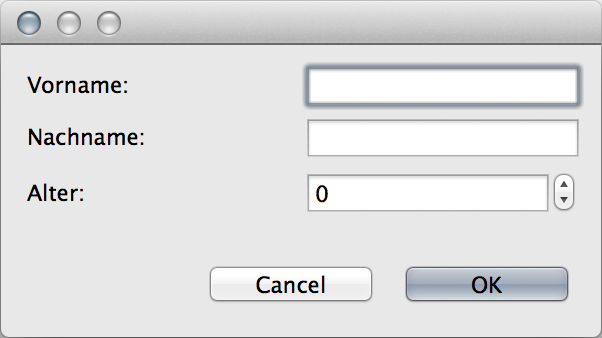
\includegraphics[width=0.5\textwidth]{person_dialog.png}
	\label{fig:proband-create}
	\caption{Neuen Proband anlegen}
\end{figure}

Nach dem Eintragen der Daten werden diese mit dem OK- Button bestätigt. 
Anschließend erscheint die angelegte Testperson auf der (linken) Seite und 
kann nun ausgewählt werden.

\begin{figure}[H]
	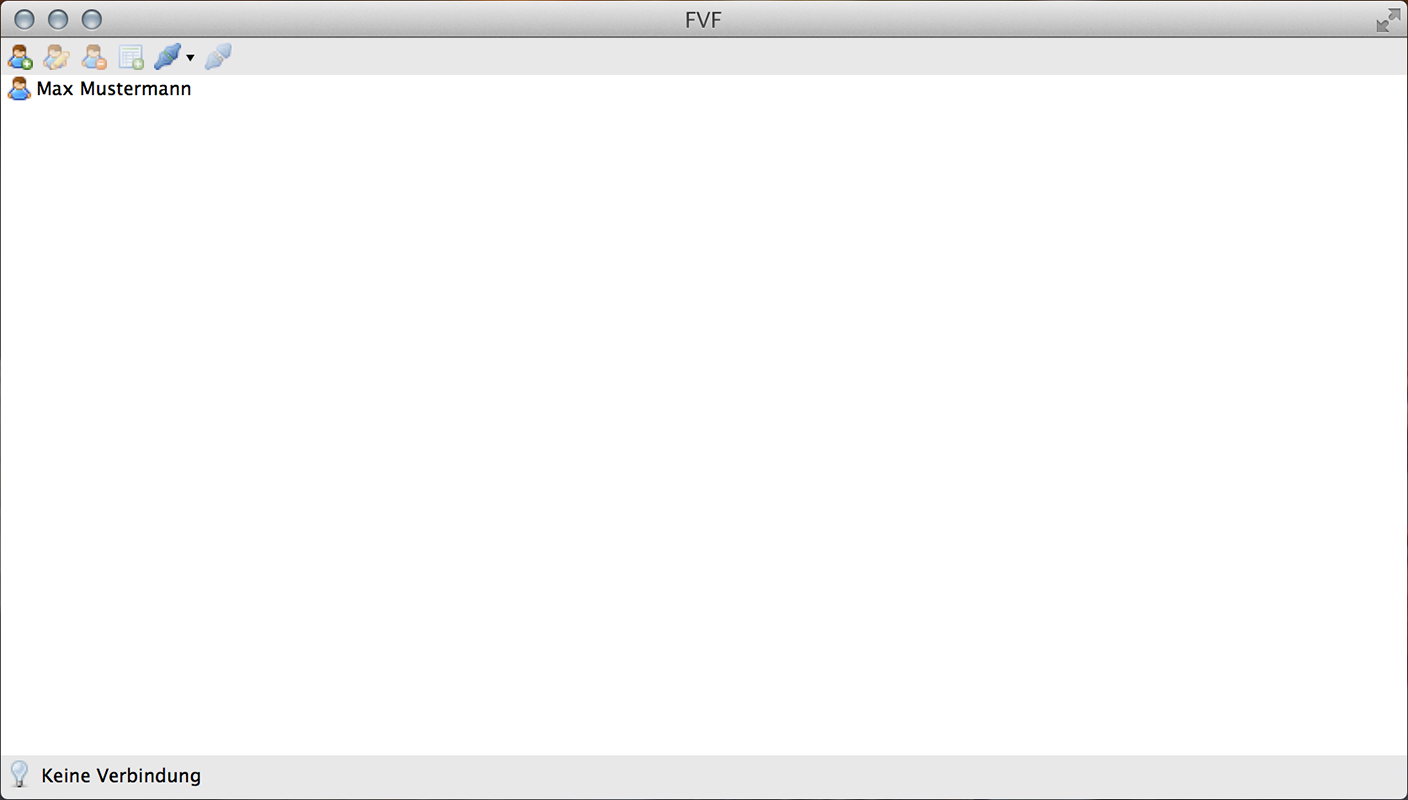
\includegraphics[width=\textwidth]{person_created.png}
	\label{fig:proband-created}
	\caption{Hauptfenster mit erstellen Probanden}
\end{figure}


\section{Proband bearbaiten}
\label{probands:proband-bearbaiten}
Durch einen Klick auf das Symbol in der Mitte, öffnet sich ein Fenster, in 
dem die eingegeben Daten einer Testperson bearbeitet werden können.

\begin{figure}[H]
	\centering
	
\includegraphics[width=0.5\textwidth]{person_edit.png}
	\label{fig:proband-edit}
	\caption{Proband bearbeiten}
\end{figure}


\section{Proband löschen}
\label{probands:proband-loschen}
Durch das Auswählen des Symbols rechts kann eine Testperson gelöscht werden. 
Durch einen Klick auf das Symbol zum Löschen erscheint wiederum das Fenster 
mit den Benutzerdaten durch das Drücken des Cancel- Buttons wird die Testperson 
gelöscht.


\section{Daten eines Probanden ansehen}
\label{probands:daten-eines-probanden-ansehen}
Die Testdaten einer Person können durch einen Doppelklick auf die Testperson 
angeschaut werden. Durch den Doppelklick öffnet sich ein Tab, in dem alle 
Testdaten eingesehen werden können.

\begin{figure}[H]
	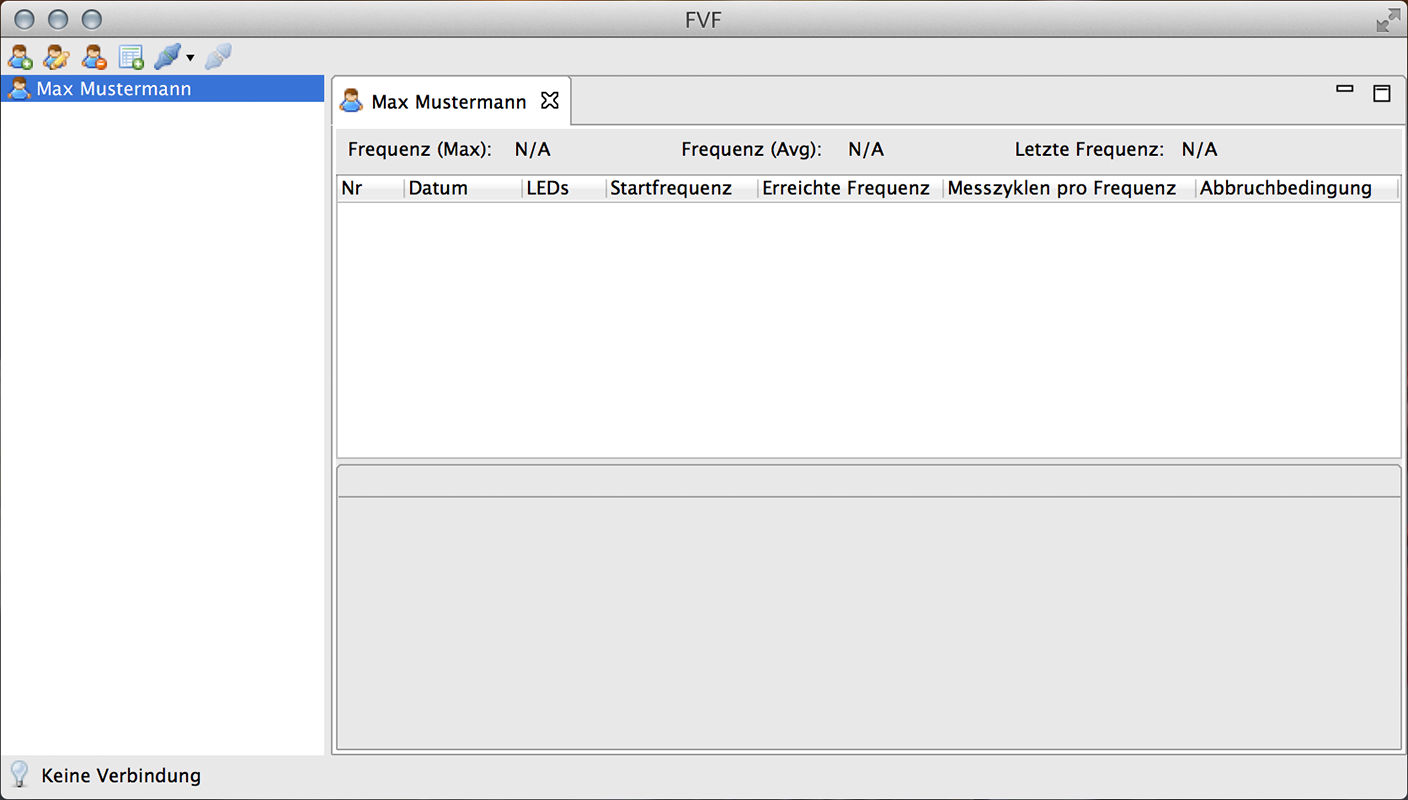
\includegraphics[width=\textwidth]{person_opened.png}
	\label{fig:proband-open}
	\caption{Proband ansehen}
\end{figure}

\chapter{Test}
\label{tests:test}\label{tests::doc}
Zum Test wird hier zuerst der 
{\hyperref[tests:test-process]{\emph{Ablauf}}} erläutert und die 
dazugehörigen {\hyperref[tests:test-parameter]{\emph{Testparameter}}} 
erklärt. Die Abschnitte {\hyperref[tests:test-new]{\emph{Neuer Test}}}}
und {\hyperref[tests:test-run]{\emph{Test Durchführen}}} beziehen 
sich auf die Eingaben für die Software.


\section{Ablauf}
\label{tests:ablauf}\label{tests:test-process}
Zu Beginn wird ein {\hyperref[tests:test-new]{\emph{Neuer Test}}} 
gestartet und die {\hyperref[tests:test-parameter]{\emph{Testparameter}}} 
müssen eingegeben werden. Der Test selbst durchläuft mehrere Frequenz-Zyklen. 
Innerhalb dieses Frequenzzyklus gibt es mehrere Messzyklen. Bei jedem Messzyklus 
flimmert eine LED, mit einer Ausnahme: Pro Frequenz-Zyklus gibt es zusätzlich 
einen Messzyklus, bei dem keine LED flimmert. Der Proband gibt ja jedem Messzyklus 
an, welche LED geflimmert hat.


\subsection{Messzyklus}
\label{tests:messzyklus}
Der Messzyklus folgt immer dem gleichen Ablauf. Zuerst werden alle LEDs 
angeschaltet und leuchten. Nach kurzer Pause werden die LEDs einzeln angeschaltet 
(wovon eine flimmert). Danach werden wieder alle angeschaltet. Das soll dem 
Probanden signalisieren, er soll seine Antwort dem Versuchsleiter mitteilen.


\subsection{Ende}
\label{tests:ende}
Der Test ist beendet, wenn der Proband zu viele Falschnennungen angegeben hat 
und damit das vorher definierte Abbruchkriterium überschritten hat oder der 
Versuchsleiter den Test abbricht.


\subsection{Durchführung}
\label{tests:durchfuhrung}
Der Versuchsleiter informiert den Probanden vor dem Start des Tests über den 
Ablauf. Die Aufgabe des Probanden ist es die flimmernde Lichtquelle zu erkennen 
und dem Versuchsleiter zu nennen. Dazu bekommt er je nach Einstellung zwei bis 
vier LEDs gezeigt, von denen pro Messzyklus nur eine flimmert. Sobald der 
Proband die flimmernde LED für sich identifiziert hat nennt er seine Antwort 
dem Versuchsleiter, der diese dann in die Messsoftware eingibt.

Während des Tests sind die zuvor eingegebenen Parameter für den Versuchsleiter 
im oberen Teil der Dialogbox zu sehen, darunter befindet sich das aktuelle 
Testprotokoll. So kann jederzeit jederzeit am Testprotokoll abgelesen werden 
welche LEDs in den vorherigen Testdurchläufen geflimmert haben, was die Antwort 
des Probanden war und ob diese richtig war. Welche die im aktuellen Messzyklus 
flimmernde LED ist, wird dem Versuchsleiter nicht angezeigt. Nach dem Beenden 
des Tests können die Ergebnisse durch das Anklicken des Buttons ``Speichern'' 
gespeichert werden.


\section{Testparameter}
\label{tests:test-parameter}\label{tests:testparameter}
Bevor der Test gestartet werden kann, müssen folgende Paramter festgelegt werden:

\begin{description}
\item[{\textbf{Anzahl der LEDs}}] \hfill \\
Der Test kann entweder mit 2 oder 4 LEDs durchgeführt werden.

\item[{\textbf{Startfrequenz {[}Hz{]}}}] \hfill \\
Legt die Frequenz für den ersten Frequenzzyklus fest.

\item[{\textbf{Frequenzsteigerung {[}Hz{]}}}] \hfill \\
Legt die Steigerung für jeden neuen Frequenzzyklus fest.

\item[{\textbf{Messzyklen pro Frequenz}}] \hfill \\
Gibt an, wieviele Messzyklen innerhalb eines Frequenzzyklus stattfinden.

\item[{\textbf{Pausendauer pro Messzyklen {[}s{]}}}] \hfill \\
Die Zeit zwischen zwei Messzyklen

\item[{\textbf{Anzeigedauer pro LED {[}s{]}}}] \hfill \\
Die Leuchtdauer pro LED

\item[{\textbf{Pausendauer pro LED {[}s{]}}}] \hfill \\
Die Dauer der Pausen zwischen den Leuchtphasen

\item[{\textbf{Abbruchkriterium (Falschnennungen)}}] \hfill \\
Ab wieviel Falschnennungen (durch den Probanden) der Test beendet wird

\item[{\textbf{Hell/Dunkel-Quotient}}] \hfill \\
Dieser Quotient bezieht sich auf die Flimmerphasen. Und zwar zu welchen Anteilen jeweils die Hell- und Dunkelphase aktiv sind.

\item[{\textbf{Bemerkungen}}] \hfill \\
Platz für Test-spezifische Bemerkungen

\end{description}


\section{Neuer Test}
\label{tests:neuer-test}\label{tests:test-new}
Zum Starten eines neuen Tests wird ``Neuer Test'' ausgewählt und es erscheint ein Fenster, in dem die Parameter für den Test eingegeben und mit \texttt{Finish} bestätigt werden.

\begin{figure}[H]
	\centering
	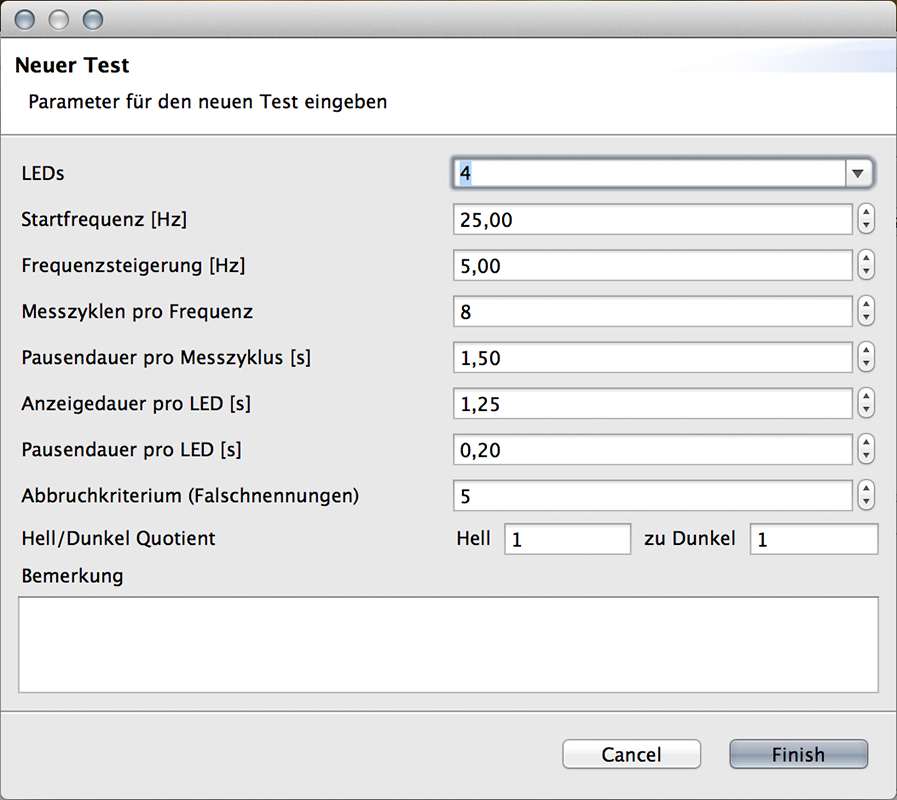
\includegraphics[width=0.8\textwidth]{test_dialog.png}
	\label{fig:test-new}
	\caption{Neuen Test erstellen}
\end{figure}

\section{Test Durchführen}
\label{tests:test-durchfuhren}\label{tests:test-run}
Nach Eingabe der Testparamter kann der Test gestartet werden. Dies geschieht durch den Button \texttt{Start} Die Antwortmöglichkeiten des Probanden können wie oben beschrieben eingegeben werden. Der Test kann jederzeit über den Button \texttt{Abbruch} abgebrochen werden, die Ergebnisse werden dann aber nicht gespeichert.

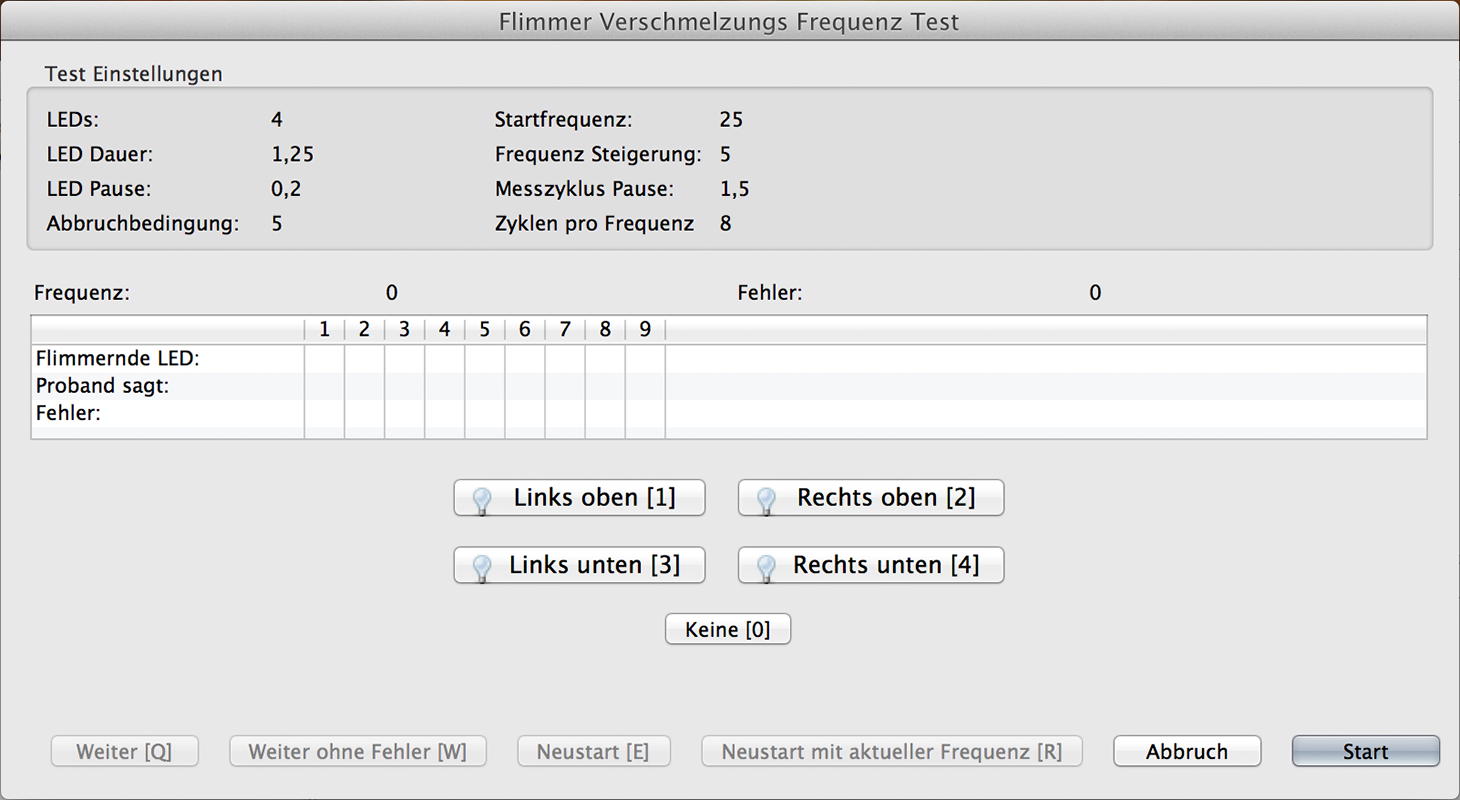
\includegraphics[width=\textwidth]{testrunner_dialog.png}

Nach dem Starten des Tests erscheint ein Fragezeichen beim jeweiligen Testdurchlauf.

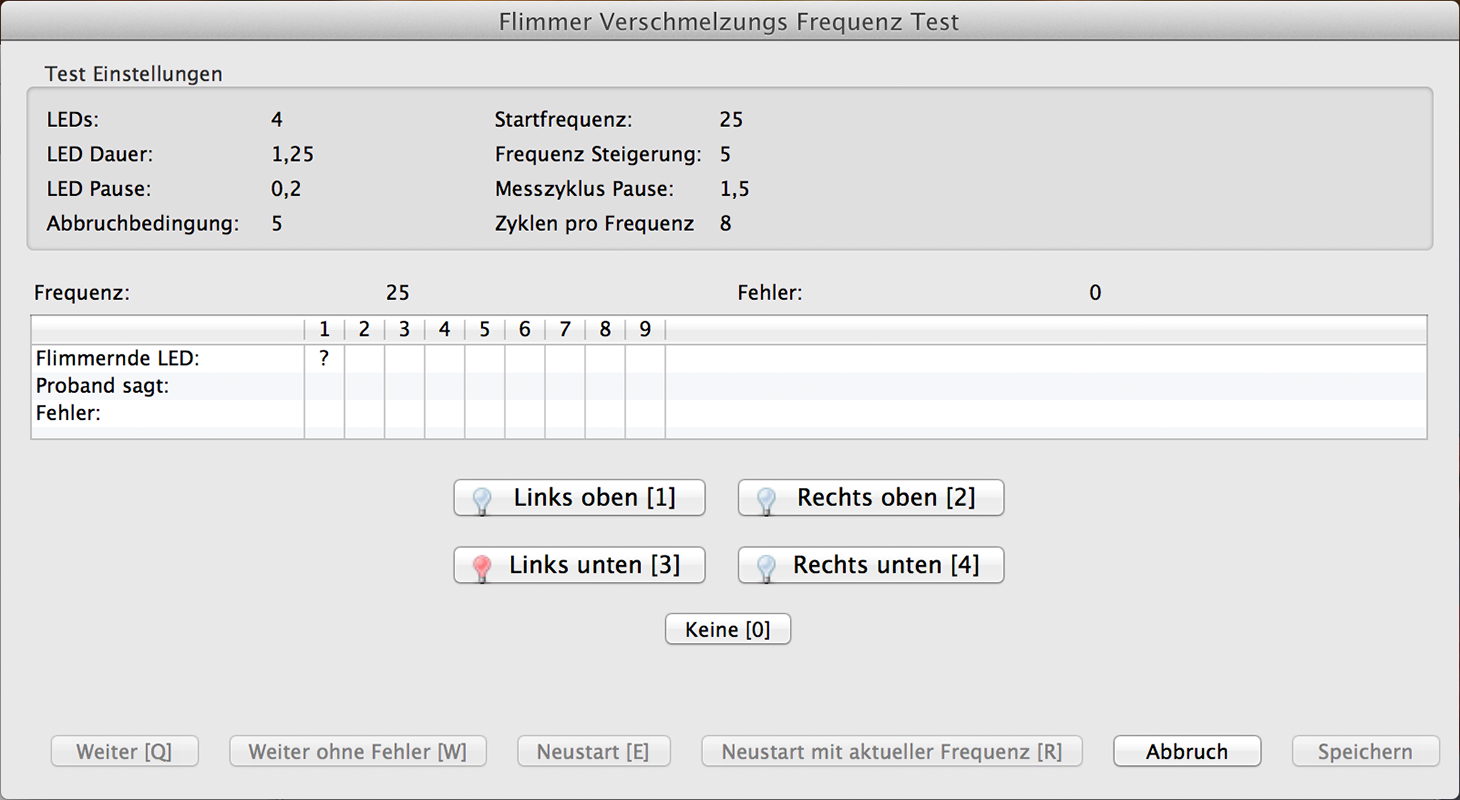
\includegraphics[width=\textwidth]{testrunner_running.png}

Nach Ende des Messzykluses sind alle LEDs und der Antwortbuttons rot gefärbt und der Versuchsleiter kann die Antwort des Probanden eingeben.

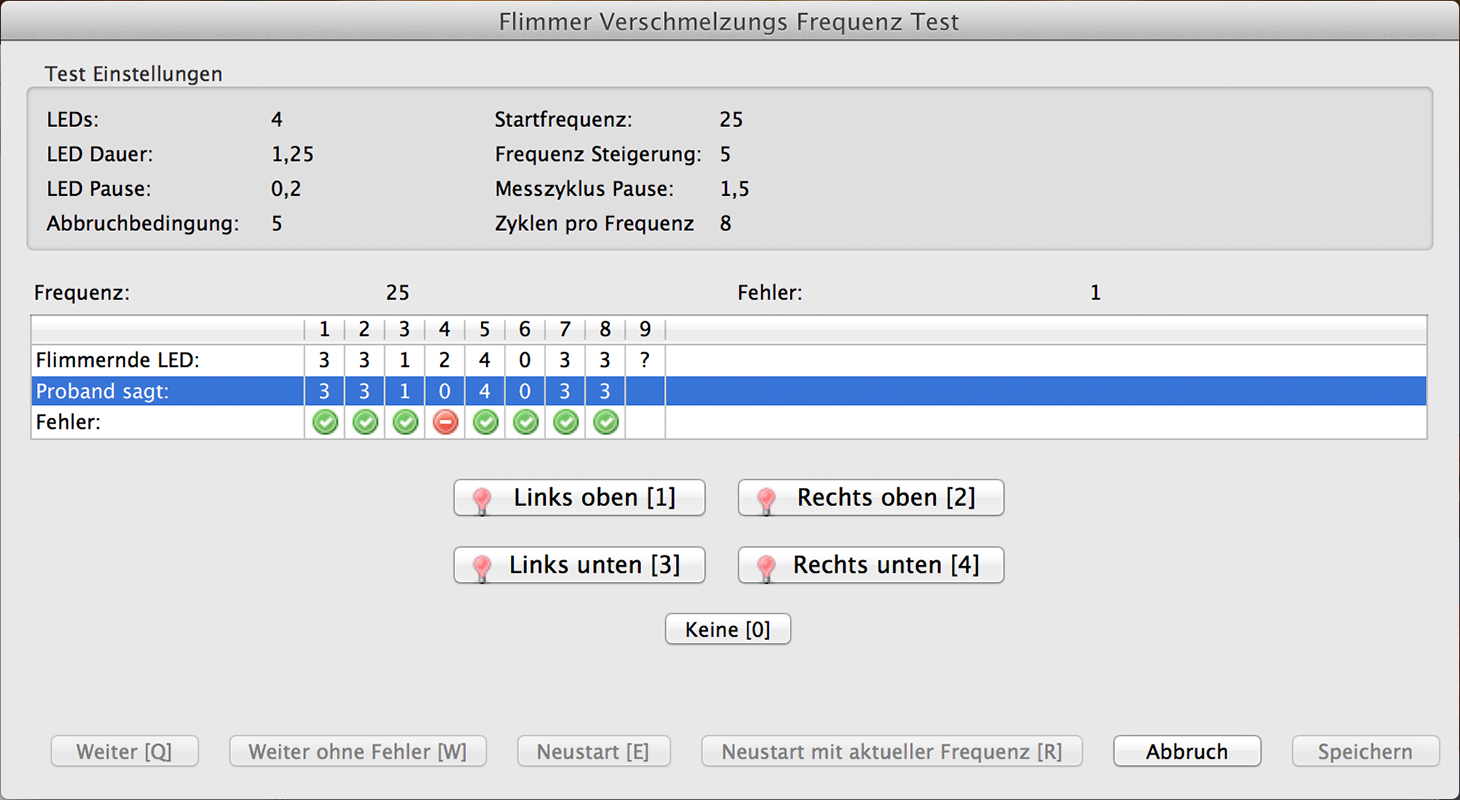
\includegraphics[width=\textwidth]{testrunner_waiting.png}


\subsection{Falsche Eingabe des Probanden}
\label{tests:falsche-eingabe-des-probanden}
Bei einer falschen Angabe des Probanden hat der Versuchsleiter mehrere Optionen wie er nun vorgehen möchte. Entweder die Buttons mit der Maus klicken oder die Taste mit dem in der eckigen Klammer stehenden Buchstaben drücken (\texttt{Q} für ``Weiter'', \texttt{W} für ``Weiter ohne Fehler'', \texttt{E} für ``Neustart'', \texttt{R} für ``Neustart mit aktueller Frequenz'').

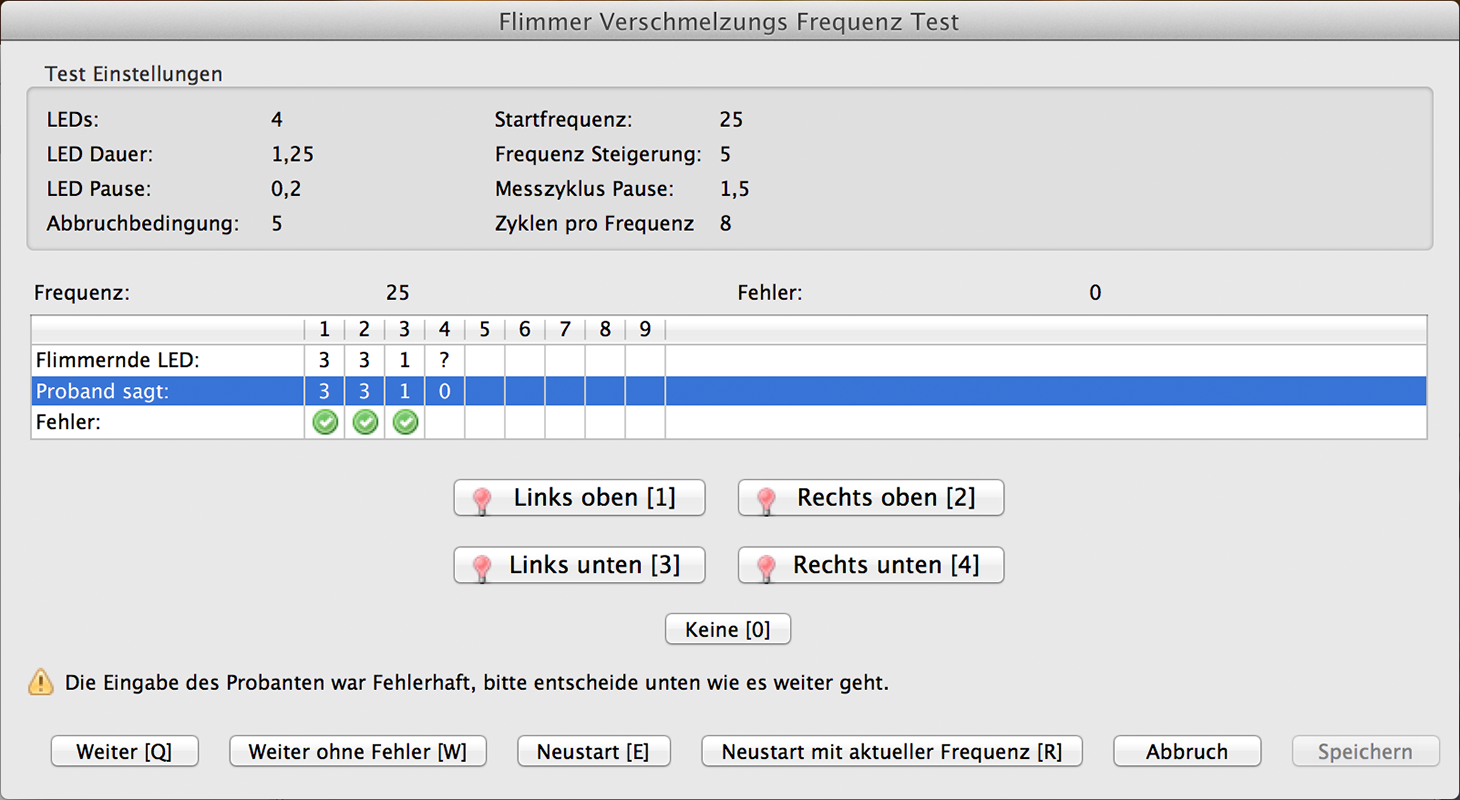
\includegraphics[width=\textwidth]{testrunner_wronganswer.png}


\subsection{Der Proband kann keine flimmernde LED benennen}
\label{tests:der-proband-kann-keine-flimmernde-led-benennen}
Wenn der Proband keine flimmernde LED mehr wahrnehmen kann und dies auch entsprechend mitteilt, wählt der Versuchsleiter die Antwort, dass keine LED geflimmert hat (z.B. die Taste \texttt{0}).


\subsection{Test beenden}
\label{tests:test-beenden}
Der Test ist beendet, wenn der Proband mehr falsche Antworten gegeben hat als vereinbart sind (Abbruchbedingung). Durch klicken des \texttt{Speichern} Buttons wird der Test gespeichert und beendet.

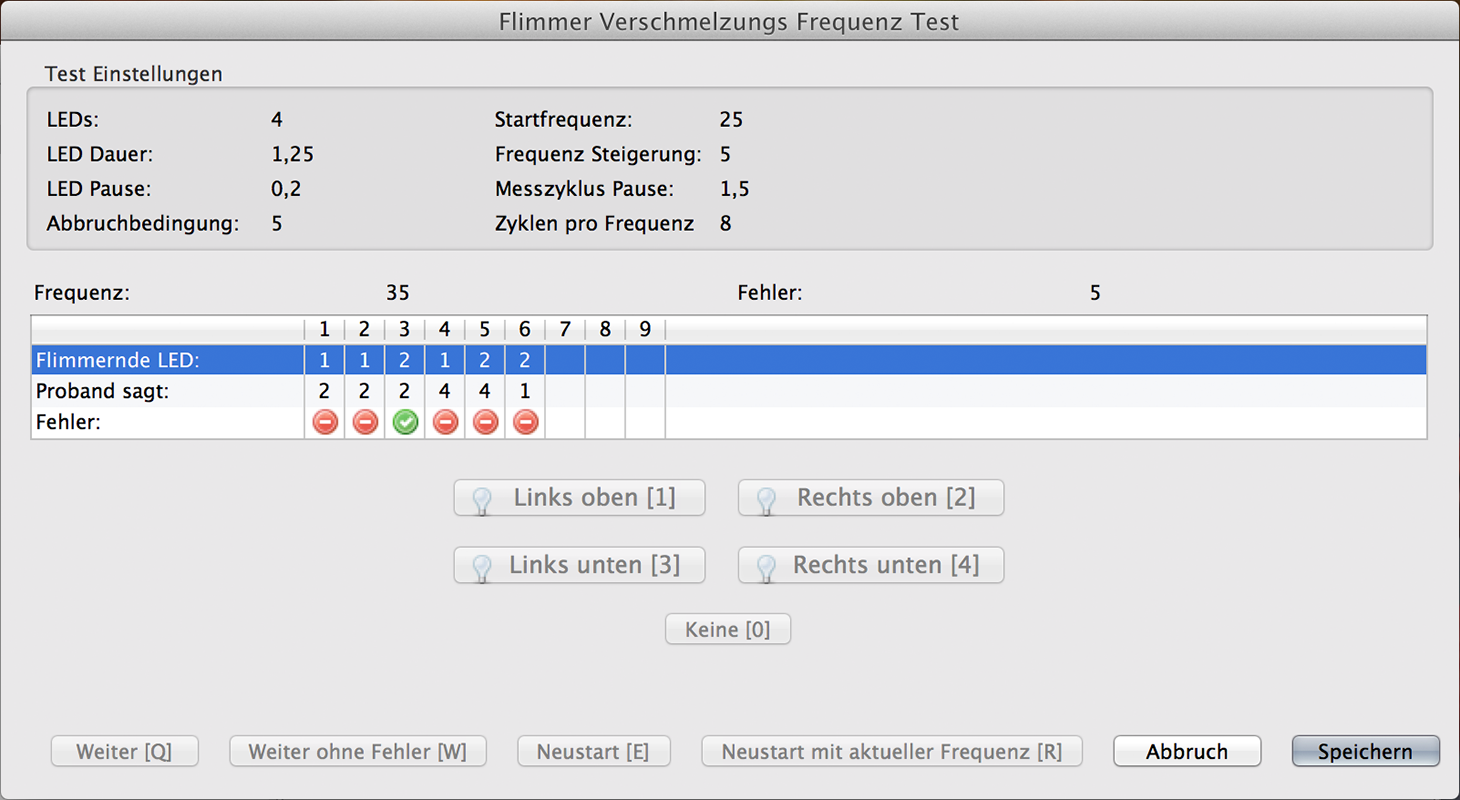
\includegraphics[width=\textwidth]{testrunner_finished.png}


\chapter{Test-Ergebnisse}
\label{results:test-ergebnisse}\label{results::doc}
Durch Doppelklicken auf eine Testperson öffnet ein Tab mit allen Daten zu der ausgewählten Testperson.
Dargstellt sind alle durchgeführten Tests und deren Ergebnisse. Durch Auswahl des gewünschten Tests und dem Fensters ``Parameter'' können sich die eingestellten Parameter des durchgeführten Tests angeschaut werden.

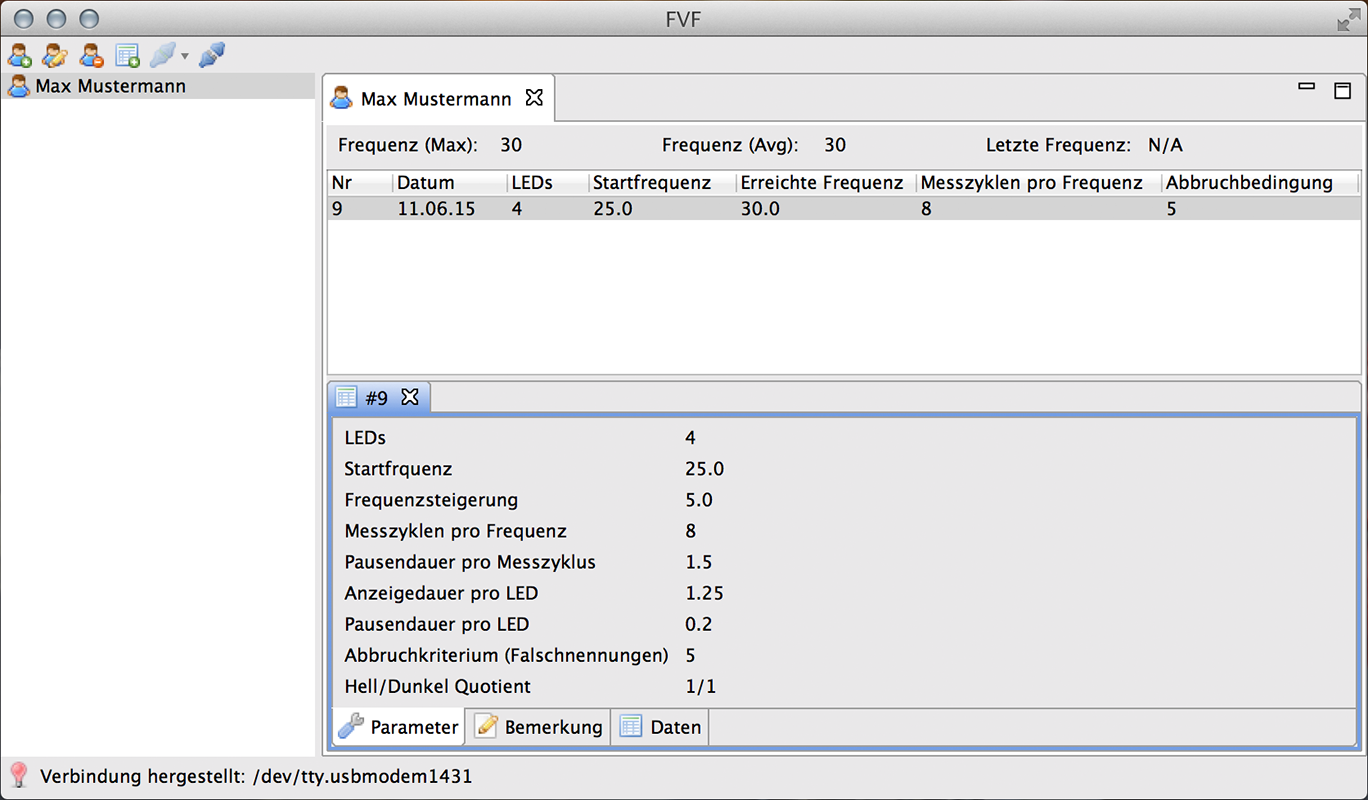
\includegraphics[width=\textwidth]{results_parameter.png}

Durch Auswahl des gewünschten Tests und dem Fenster ``Bemerkung'' können sich Bemerkungen zu dem durchgeführten Test angeschaut werden.

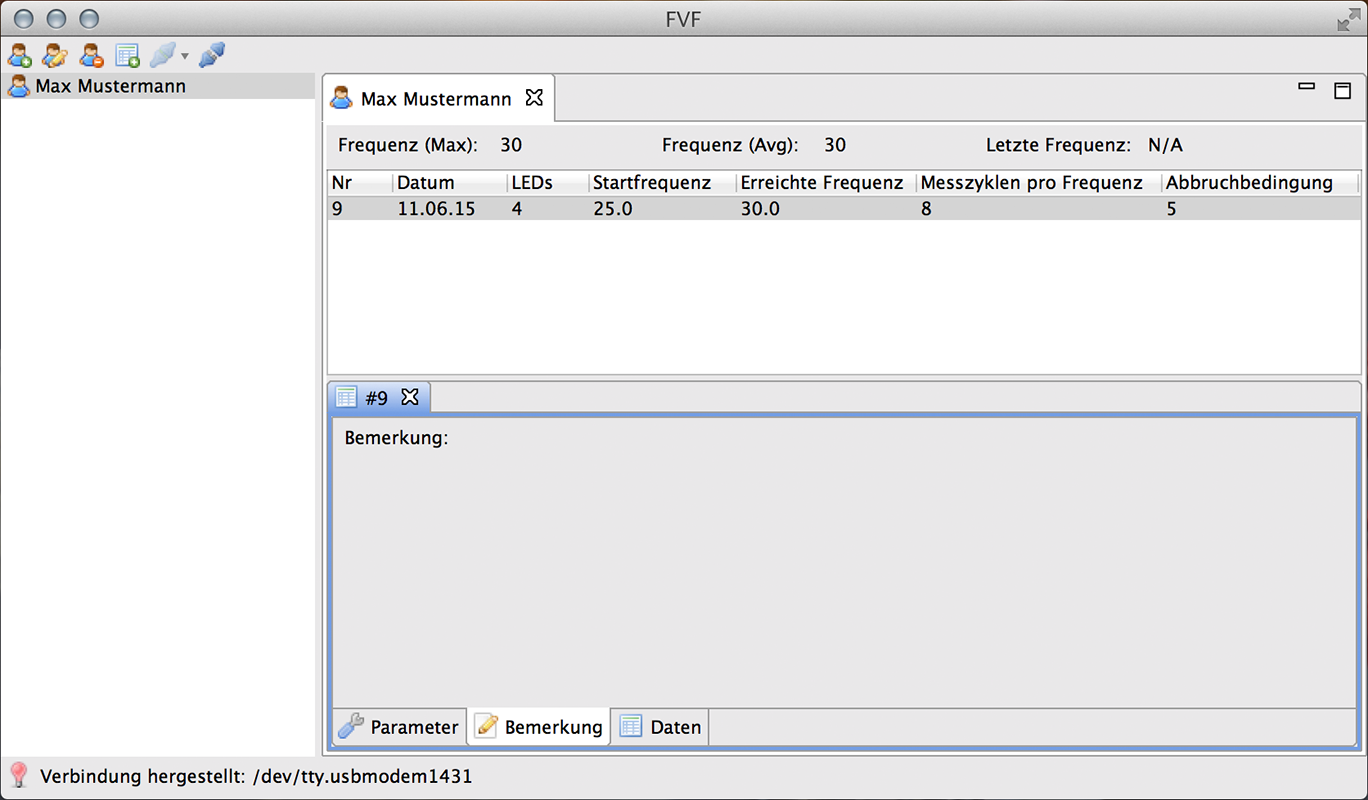
\includegraphics[width=\textwidth]{results_notes.png}

Unter ``Daten'' können sich dei einzelnen Daten zu einem Test angeschaut werden. Hier ist aufgelistet ind welcher Frequenz die LED geflimmert hat, welche Antwort der Proabnd gegeben hat und welche die flimmernde LED war und ob die Antwort des Probanden richtig oder falsch war.

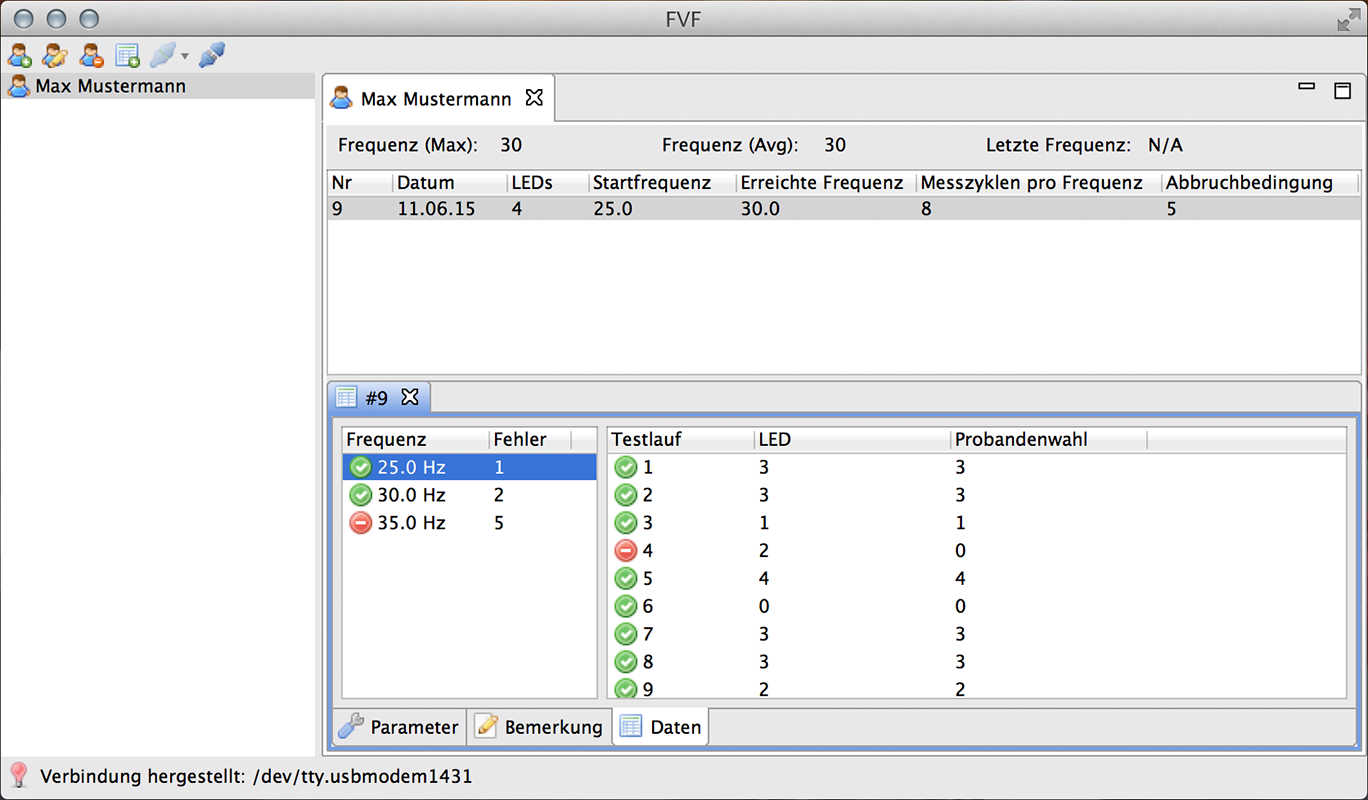
\includegraphics[width=\textwidth]{results_runs.png}


\chapter{Literatur}
\label{references::doc}\label{references:literatur}
Wiemeyer, J. (2001). Flimmerverschmelzungsfrequenz. Ein multifaktorieller psychophysischer Indikator im Sport. \emph{Zeitschrift für praktische Augenheilkunde \& augenärztliche Fortbildung}, S. 426-432.

\end{document}
			